
\section{Figures and Tables}

\begin{figure}[h!]\centering
\begin{minipage}{0.49\textwidth}
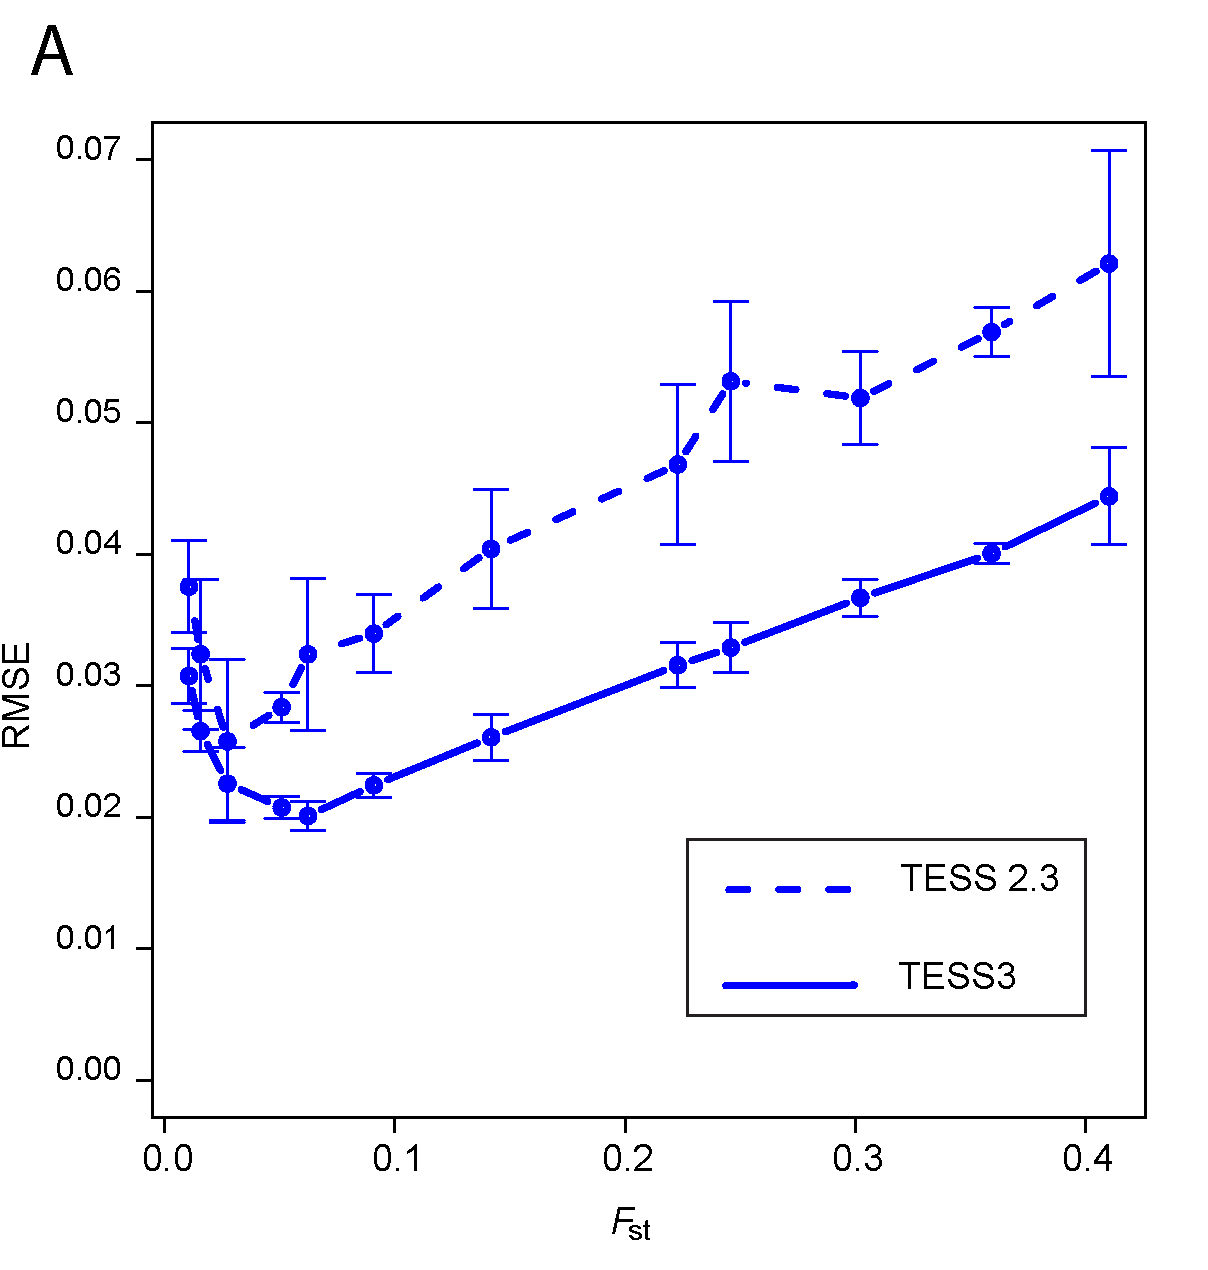
\includegraphics[width=\linewidth]{FinalGraphs/rmseG.pdf}
\end{minipage}
\begin {minipage}{0.49\textwidth}
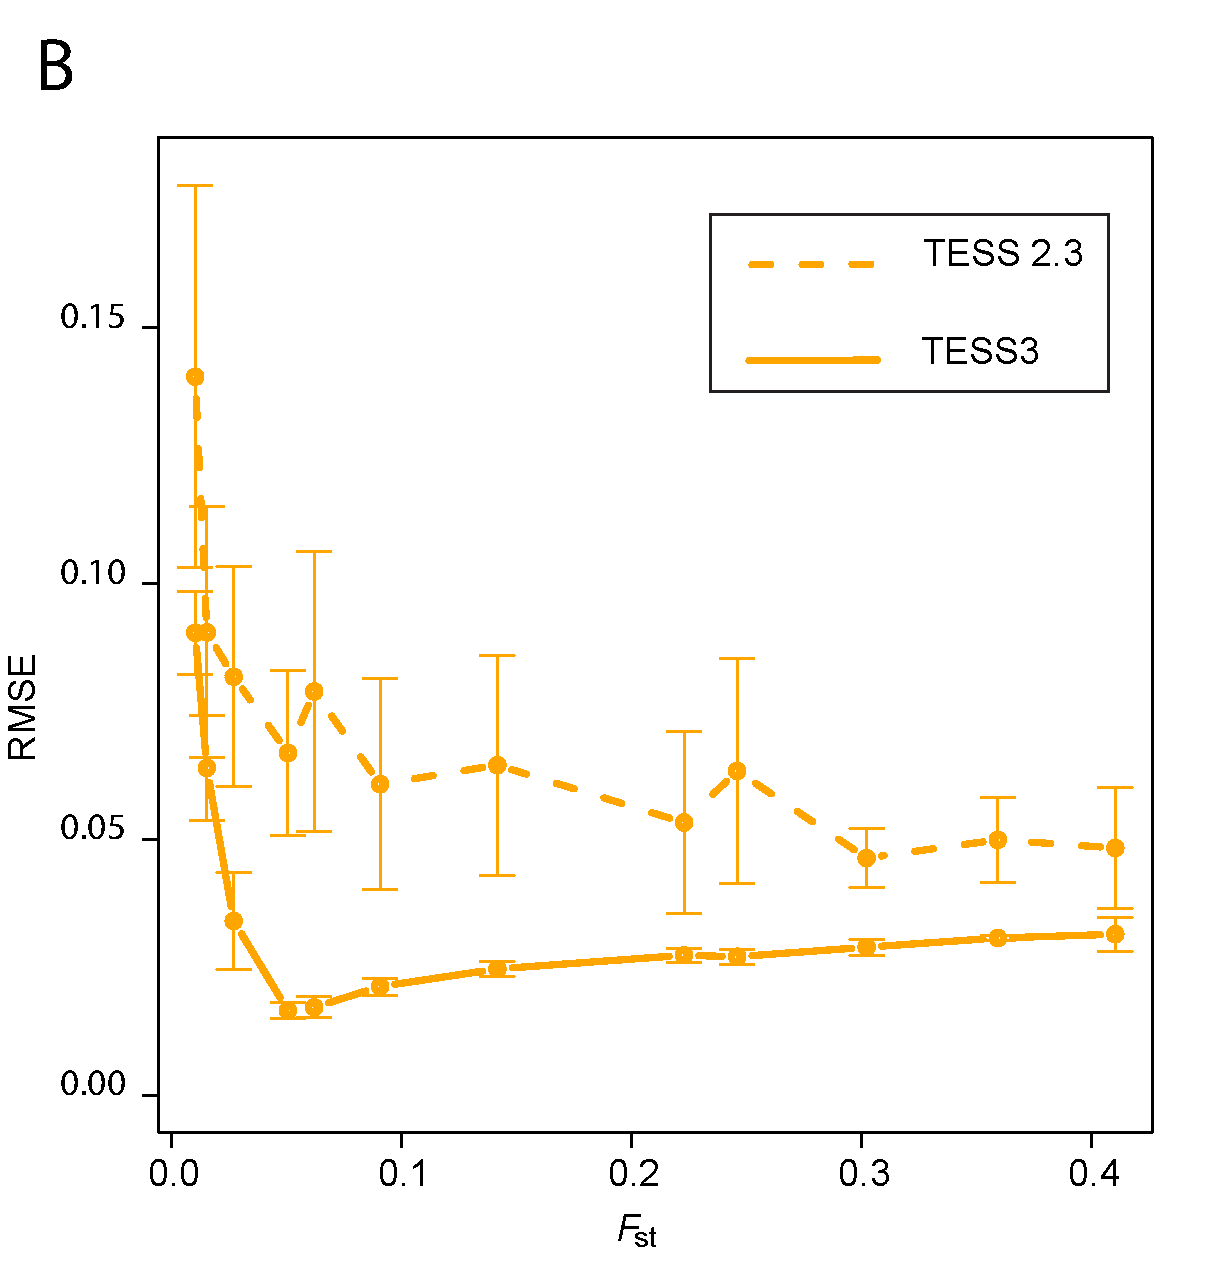
\includegraphics[width=\linewidth]{FinalGraphs/rmseQ.pdf}
\end{minipage}
\caption{Statistical errors of {\tt TESS3} and {\tt TESS 2.3} estimates. Computer simulations of admixed populations using known individual ancestry proportions from two ancestral gene pools. A) RMSEs of $G$ estimates as a function of the level of ancestral population differentiation ($F_{\rm ST}$). B) RMSEs of $Q$ estimates as a function of the level of ancestral population differentiation ($F_{\rm ST}$).}
\end{figure}    

\clearpage
\newpage



\begin{figure}[h!]
  \centering

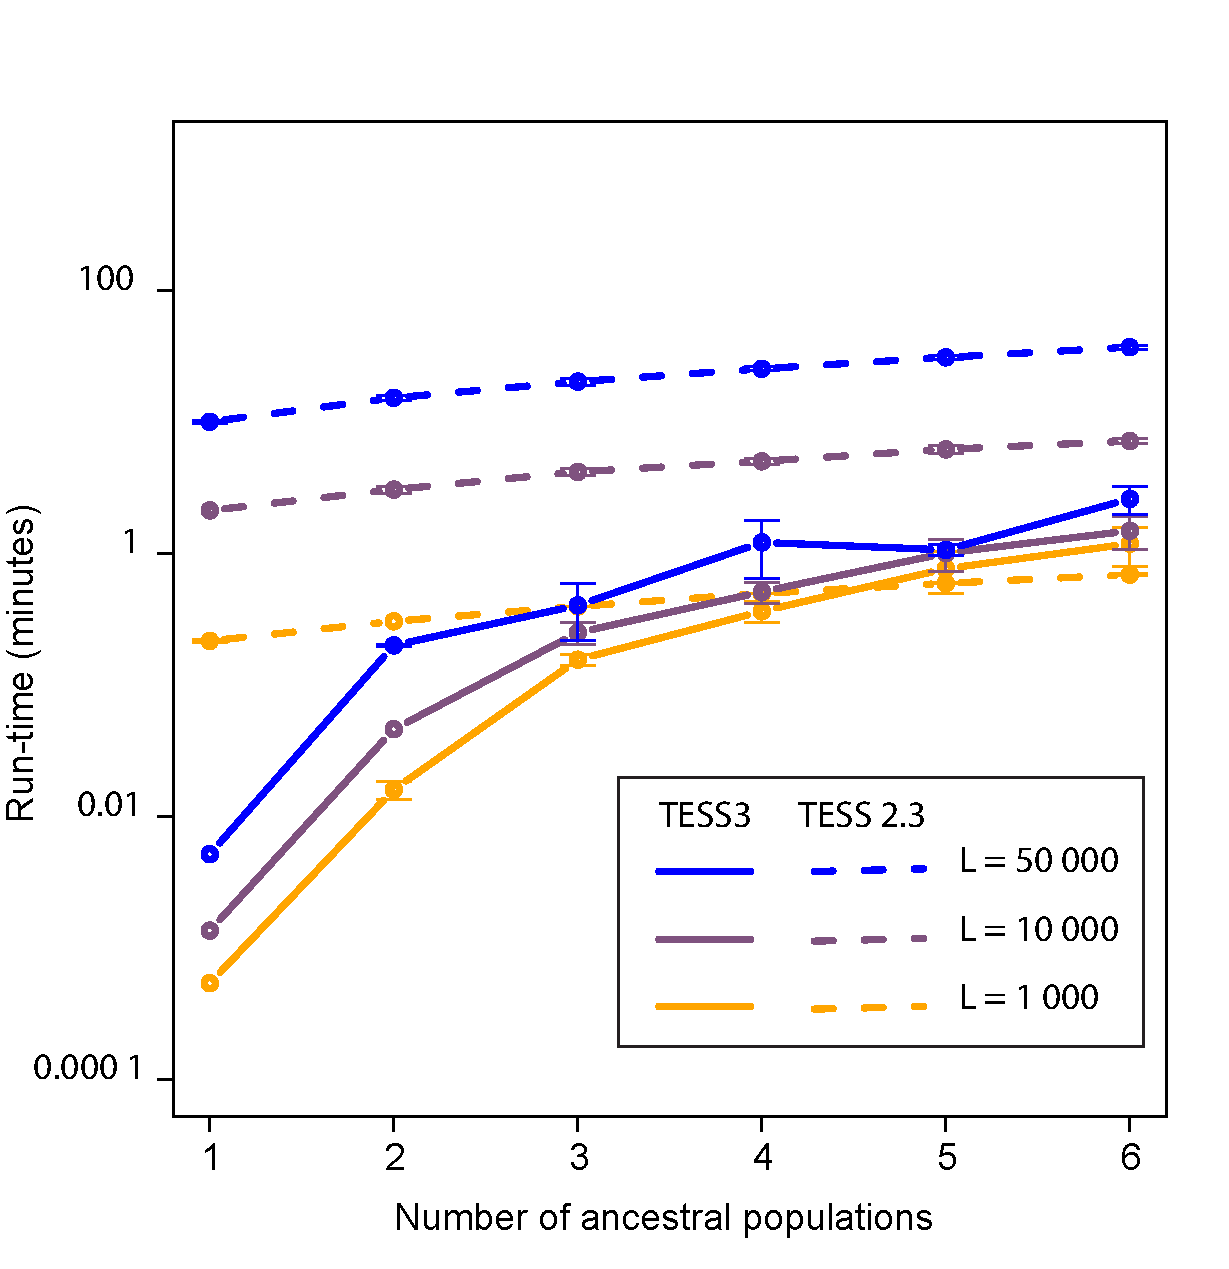
\includegraphics[width=\linewidth]{FinalGraphs/runtimes.pdf}
\caption{ Run-times for {\tt TESS3} and {\tt TESS 2.3} for numbers of ancestral populations ranging between $K = 1$ and $6$. Runtimes were expressed in unit of minutes. }
\end{figure}

\clearpage
\newpage

\begin{table}
\begin{center}
\begin{tabular}{lcc}
 \hline
\textbf{FDR}  & \multicolumn{2}{c}{\textbf{Power}}  \\
 & $m_{\rm s} / m = 0.005$ & $m_{\rm s} / m = 0.05$ \\
\hline
 0.050 & 0.61& 0.16 \\
 0.10 & 0.63 & 0.17\\
 0.15 & 0.64 & 0.19 \\
 0.20 & 0.65 & 0.20 \\
 \hline
\end{tabular}
\end{center}
\caption{Power to reject neutrality for two simulated data sets with distinct values of the ratio ($m_{\rm s} / m$).}
\end{table}


\clearpage	
\newpage


\begin{figure}[h!]\centering
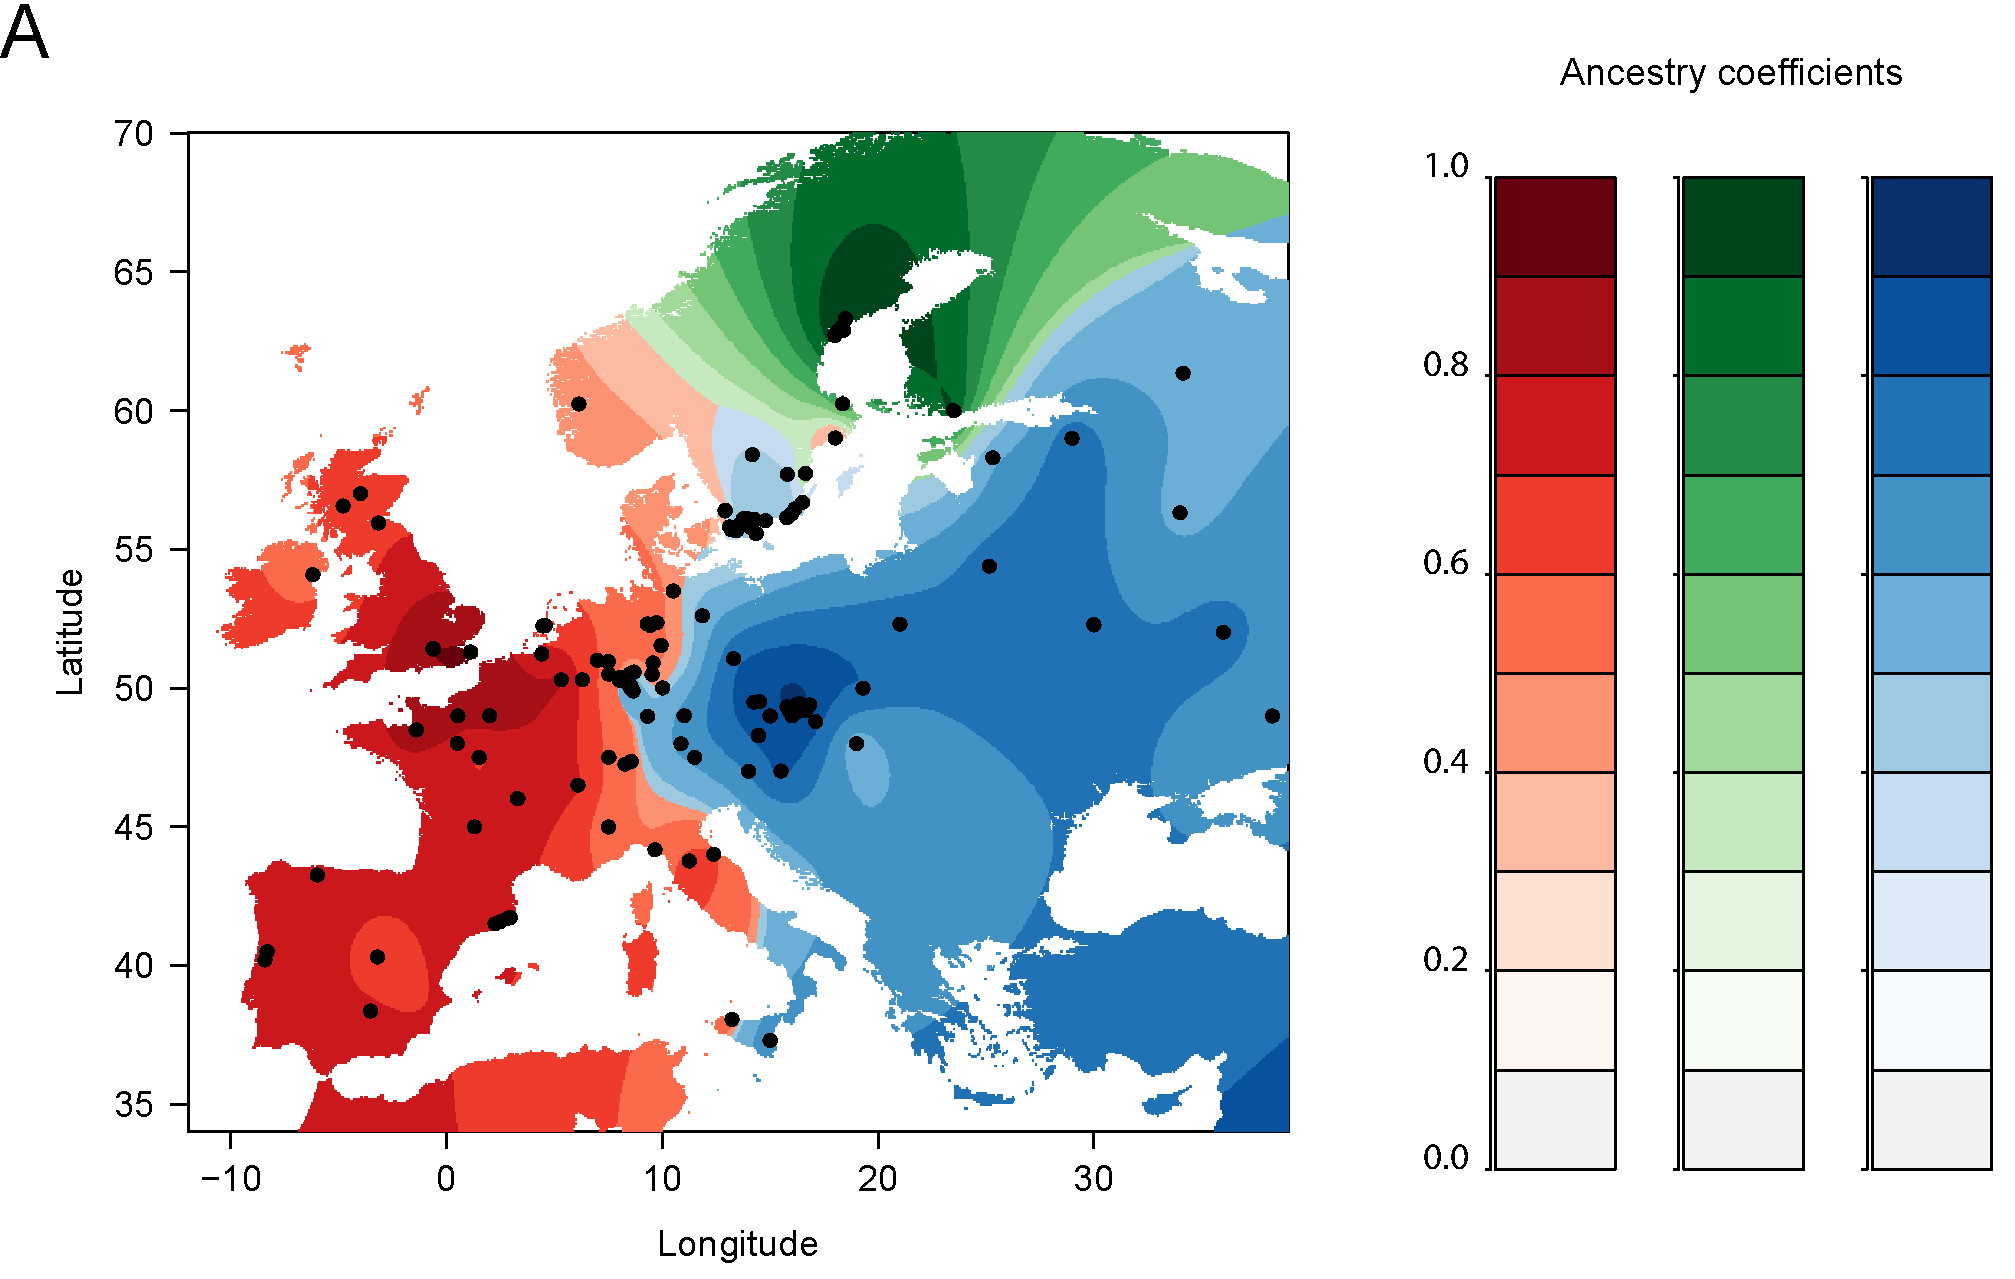
\includegraphics[width=\linewidth]{FinalGraphs/barsClusters.pdf}
\includegraphics[width=\linewidth]{FinalGraphs/manhattanPlot.pdf}
\caption{Results of the {\it Arabidopsis thaliana} data analysis with {\tt TESS3}. A) Geographic maps of ancestry coefficients using $K = 3$ ancestral populations. C) Manhattan plot for the chromosome 5. The horizontal line corresponds to an expected FDR value of $q = 10^{-30}$. }
\end{figure}    

\clearpage
\newpage 

\begin{figure}[h!]\centering
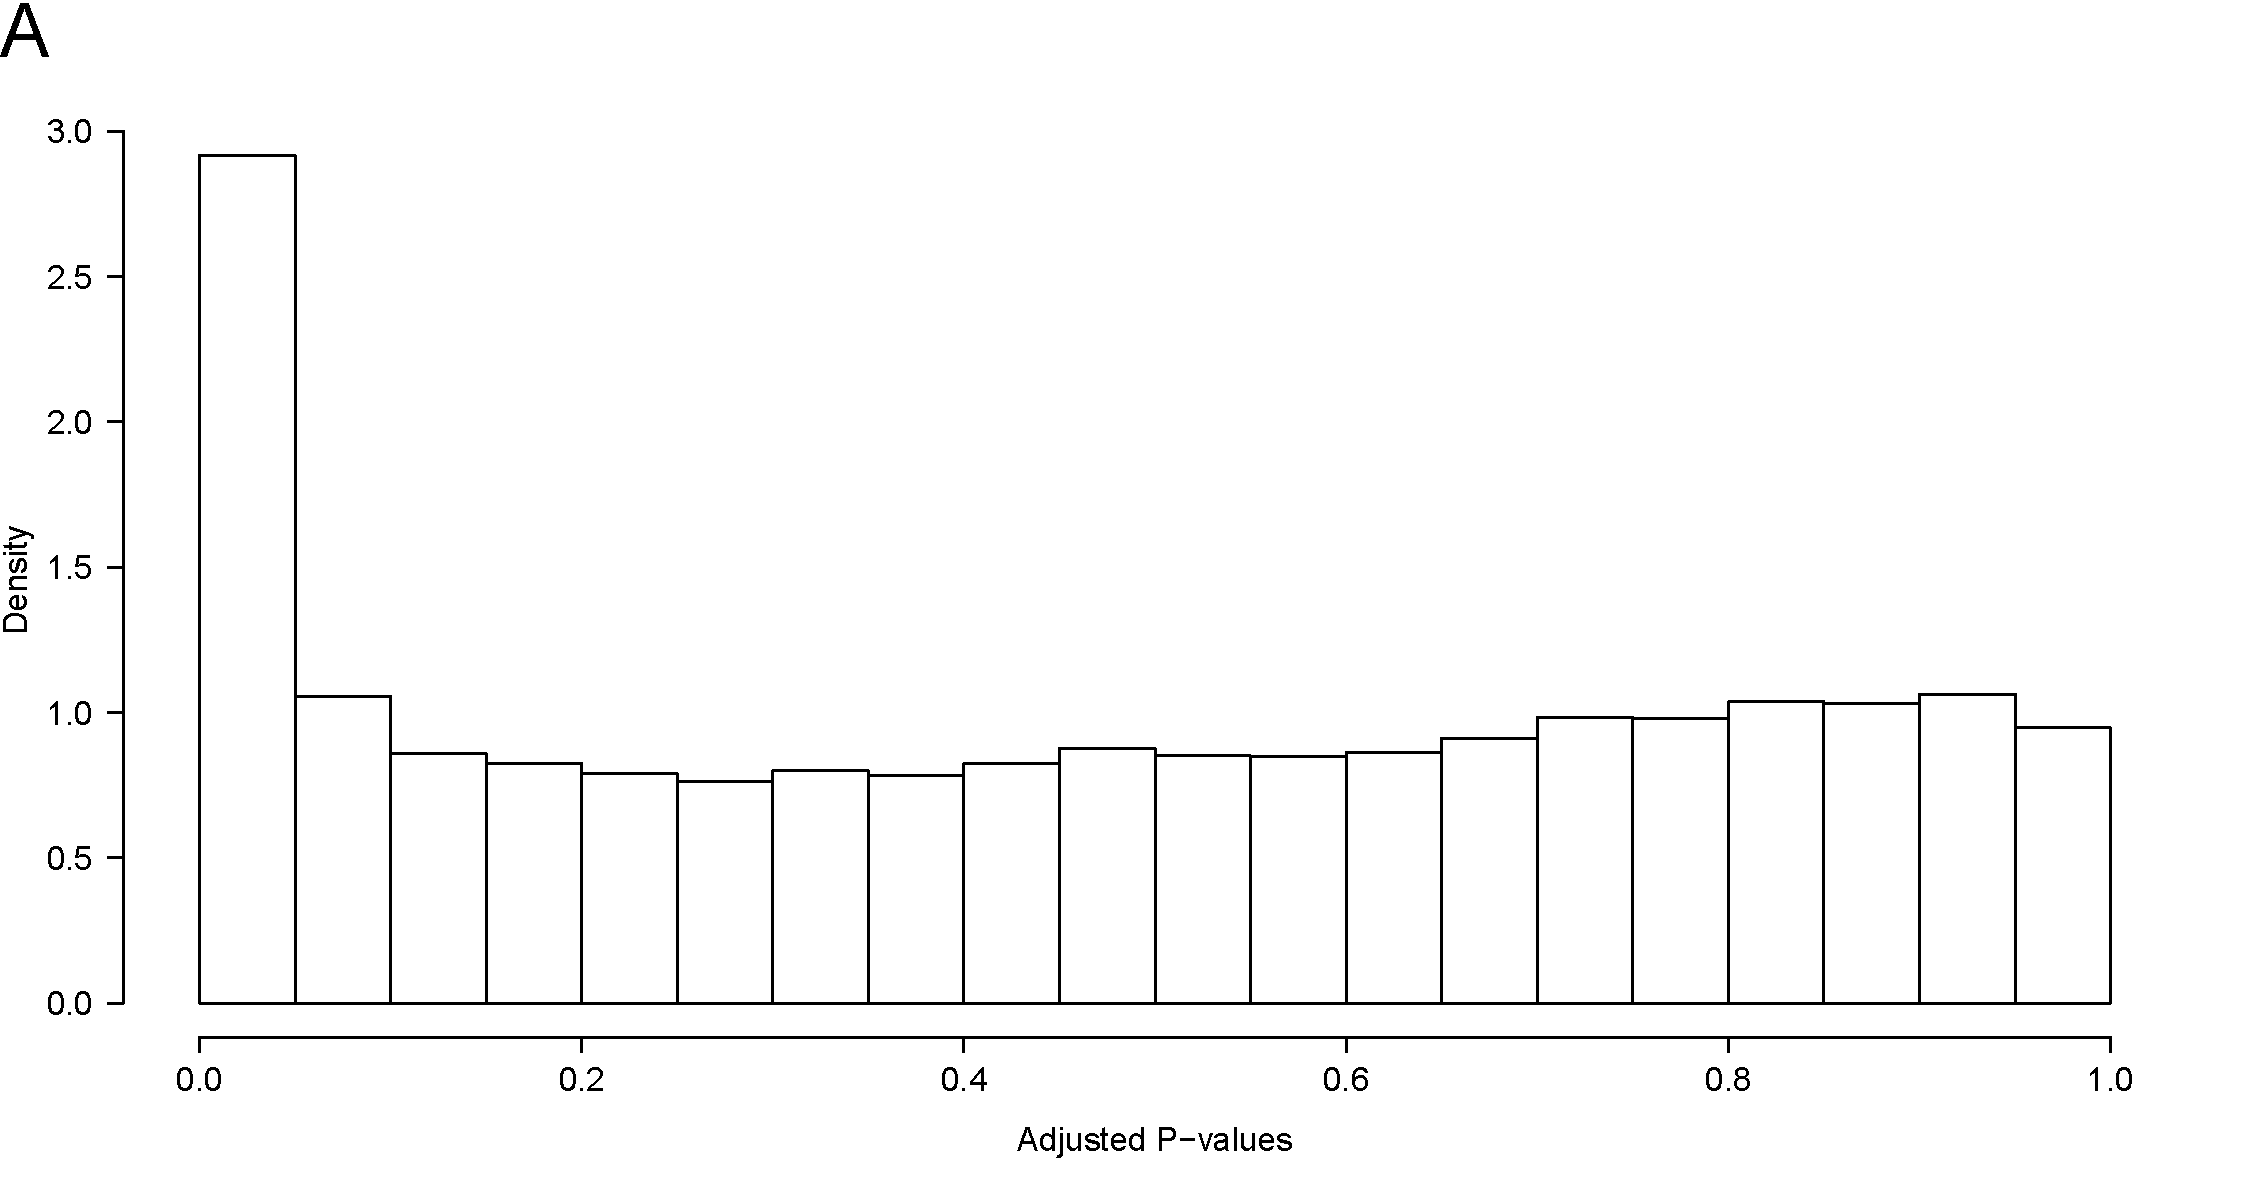
\includegraphics[width=\linewidth]{FinalGraphs/pValueHist.pdf}
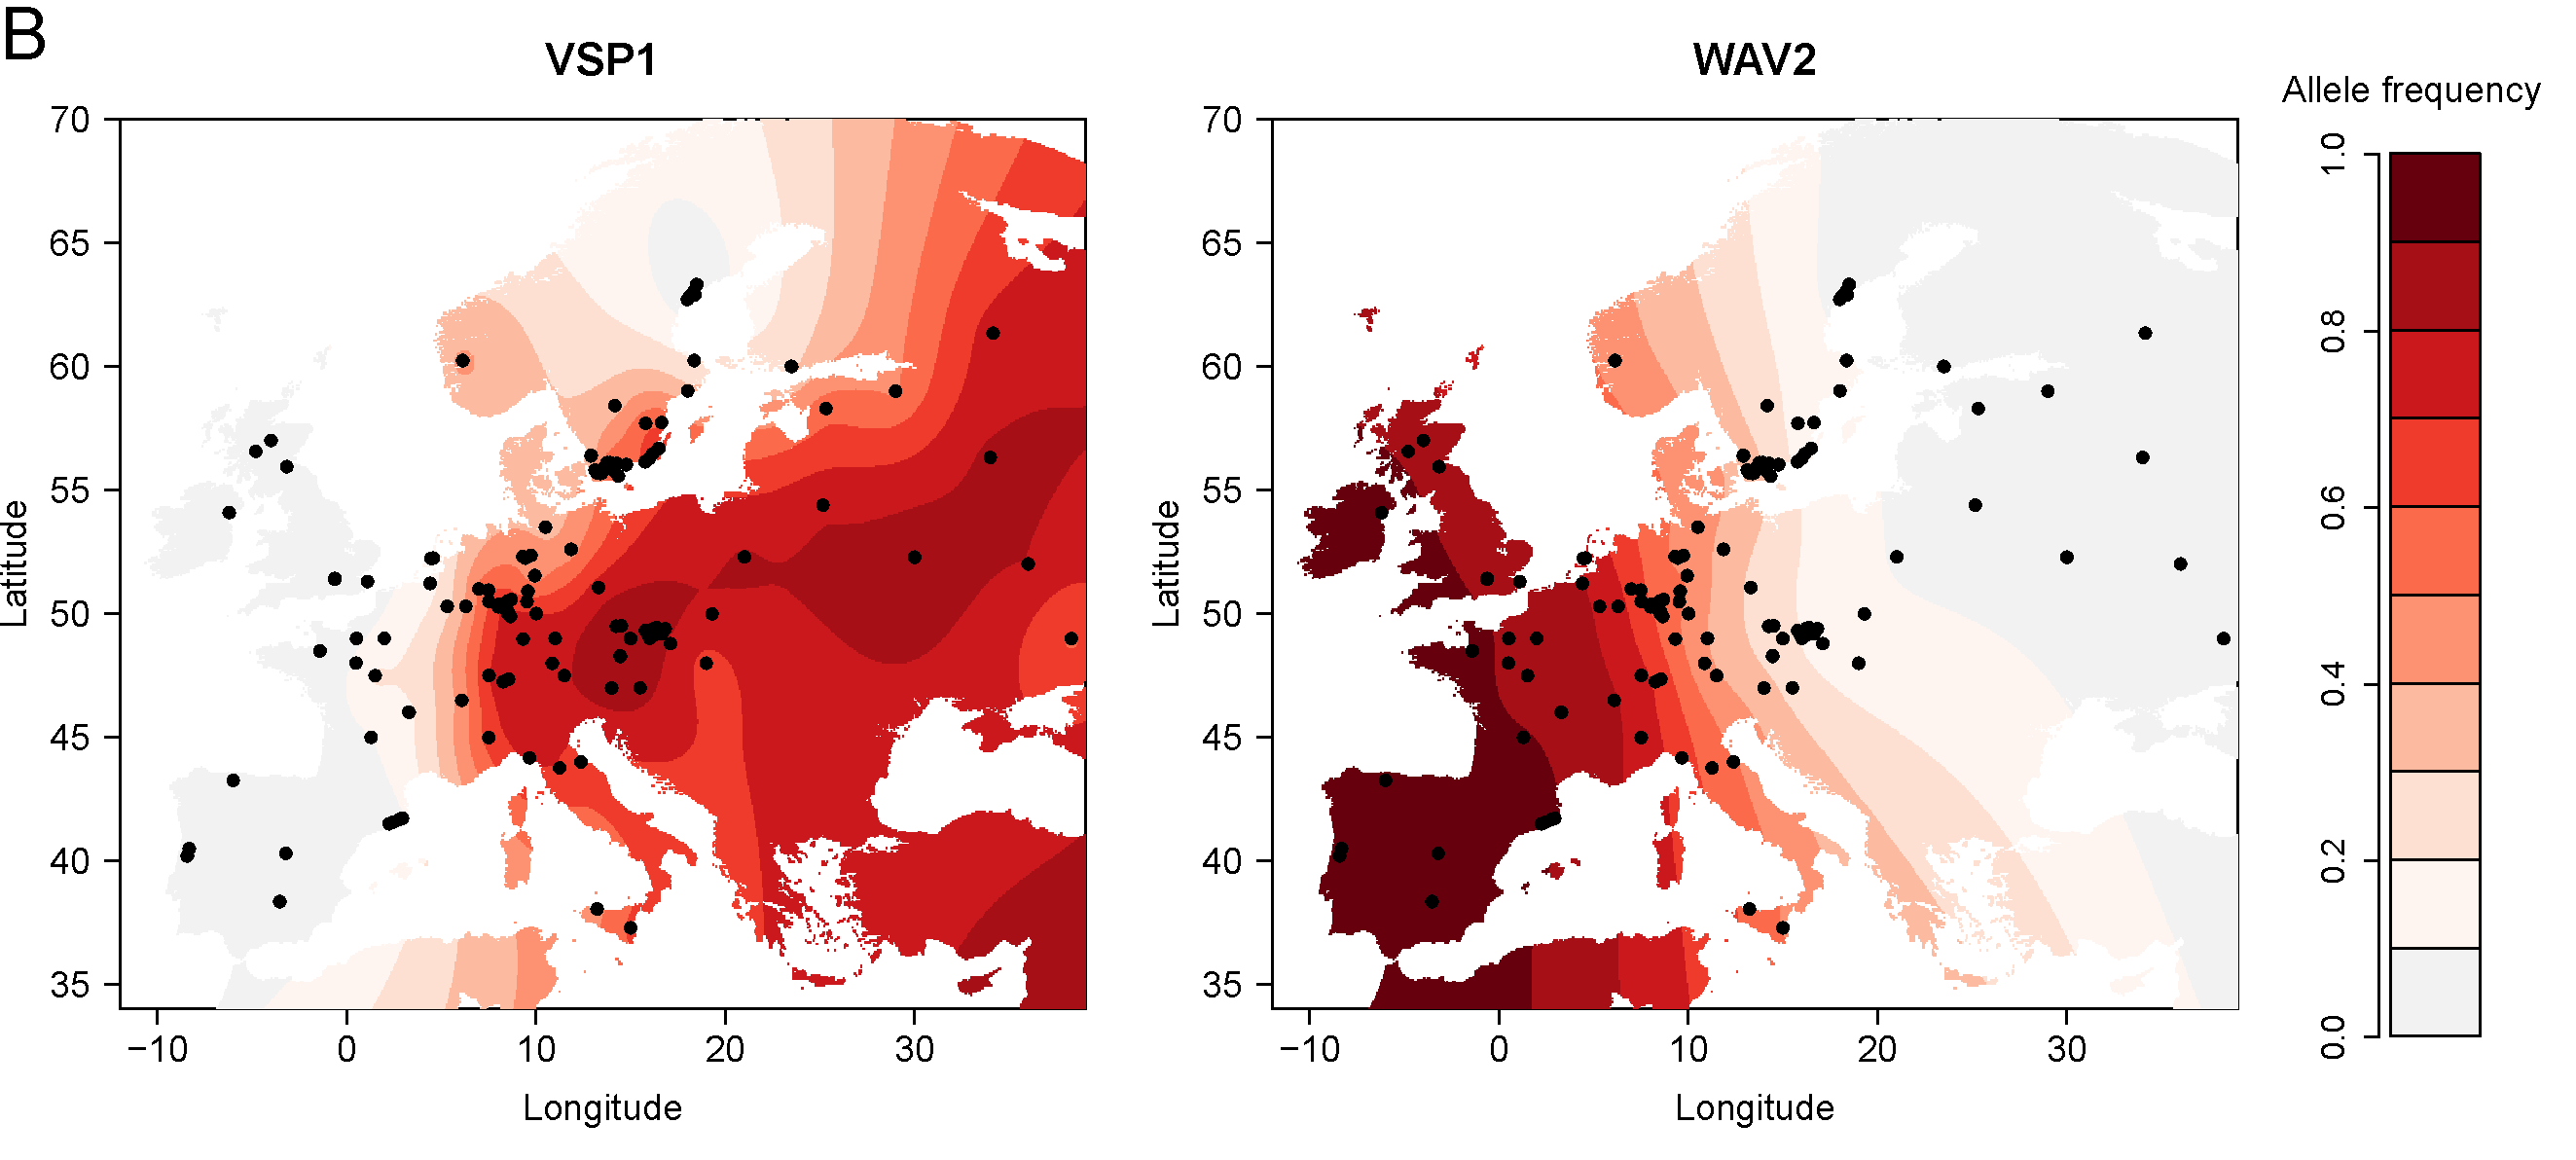
\includegraphics[width=\linewidth]{FinalGraphs/colorBar.pdf}
\caption{ Discoveries from a scan of the {\it A. thaliana} 5th chromosome. A) Histogram of adjusted $p$-values. B) Spatial distribution of two top-hit SNPs located in the {\it VSP1} and {\it WAV2} genes.}
\end{figure}    


\clearpage
\newpage 
